\section{Halbmetalle und Halbleiter}
Halbmetalle: B, Si, Ge, As, Se, Sb, Te, Po, At \\

Halbmetalle zeigen keine einheitlichen Stoffeigenschaften und keinen einheitlichen Aufbau. \\

\subsection{Halbleiter}
Stoffe mit geringer el. Leitfähigkeit, welche bei steigender Temperatur zunimmt. Halbmetalle sind Halbleiter, aber nicht jeder Halbleiter ist ein Halbmetall. \\

Im Energiebänder-Modell: kleine Verbotene Zone zwischen Valenz- und Leitungsband, ca. 0-3 eV (Si: 1.12 eV bei 300K) \\

Bei steigender Temperatur: Zufuhr von Energie $\Rightarrow$ $e^-$ aus Valenzband kann ins leere Leitungsband springen und hinterlässt Lücke im Valenzband = \emph{Defektelektron}.

\begin{figure}[htbp]
	\centering
	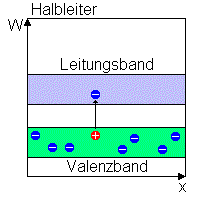
\includegraphics[width=0.4\linewidth]{images/4_Halbleiter_Energiebaender.png}
\end{figure}

\subsection{Dotierung}
Einbringen von Fremdatomen zur Veränderung der elektrischen Eigenschaften.

\subsubsection{n-Halbleiter}
El. Leitung v.a. durch $e^-$. \\

Bsp. Dotierung von Si mit As: 1 As-Atom pro $10^7$ Si-Atome. $\Rightarrow$ 1 schwach gebundenes Valenz-$e^-$ pro As-Atom $\Rightarrow$ Steigerung der Leitfähigkeit um Faktor $10^6$. \\

5. Valenz-$e^-$ entspricht einem vollen Energieband (Donatorband) knapp unterhalb des Leitungsbands. \\

\subsubsection{p-Halbleiter}
El. Leitung v.a. durch (positive) Defektelektronen. \\

Bsp. Dotierung von Si mit B: 1 B-Atom pro $10^6$ Si-Atome. $\Rightarrow$ 1 fehlendes $e^-$ pro B-Atom $\Rightarrow$ Defektelektron (\emph{Loch}) kann von Si-Valenz-$e^-$ besetzt werden $\Rightarrow$ positive Löcher. \\

Defektelektron entspricht leeren Energieband (Akzeptorband) knapp oberhalb des Valenzbandes.